%TODO remove draft
\documentclass[11pt,a4paper]{article}

\usepackage{graphicx}
\title{Genetic Algorithms}
\author{Alexander D Brown (adb9)}

\begin{document}
\maketitle
\tableofcontents

\newpage
\section{Introduction}
Genetic algorithms are a biologically-inspired approach to heuristic search 
which mimic natural selection. Unlike many other evolutionary strategies and
evolutionary programming, they are not designed to solve a specific problem,
but are designed to solve the problem of optimisation which is made difficult
by substantial complexity and uncertainty\cite{Holland1992Adaptation}.

The complexity of the task should make it such that discovering an optimum
solution is a long, maybe even impossible, task. At the same time the 
uncertainty needs to be reduced so that the knowledge of \textit{available}
options can be increased.

% TODO improve this section as its mainly from the reference.
The initial design for a genetic algorithm was a method for moving from one
population of chromosomes to another using a form of natural selection. This
algorithm also included methods for crossover, mutation and inversion. This
idea of having a large population was the distinguishing feature from any past
attempts which had only considered the parent and one offspring, where the 
offspring was simply a mutation of the parent\cite{Mitchell1996Introduction}.


\subsection{Evolutionary Algorithms}
As their name suggests, an evolutionary algorithm applies elements from the 
biological theory of evolution to the problem of optimisation. These elements
include:

\begin{itemize}
\item Reproduction
\item Mutation
\item Recombination
\item Selection
\end{itemize}

Typically, a population of candidate solutions are generated to which a fitness
function can be applied. The population is then subject to some form of 
evolution, and this process is repeated until a halting criteria is met.

Genetic algorithms are a type of evolutionary algorithm with a focus on the 
genetic evolution of solutions. Candidate solutions for genetic algorithms, 
known as \textit{chromosomes} are encoded as a series of \textit{genes}. These
genes are a representation of the choices which need to be optimised for the 
solution and can be as simple as a single bit or as complex as a real number, 
depending on the problem.

There are many other forms of both evolutionary and genetic algorithms which
this report with mention in later sections.


\newpage
\section{Basic Genetic Algorithm Principals}
The basic principals of genetic algorithms are to represent candidate solutions
as a population of chromosomes, from this population the fittest members can be
picked out and used in the next generation and to create new member of the 
population through reproduction and/or mutation.

This cycle repeats with the aim to produce better performing individuals in 
each generation until the optimum solution is either reached or gotten close
enough to that any future improvement is unnecessary or unwanted due to
other constraints such as processing time. The latter of these allows a genetic
algorithm to come up with a ``good'' solution in a reasonable amount of time.

Reproduction and mutation are an important part of genetic programming, and too
of evolutionary programming. Without these parts the algorithm would quickly 
reach a local optima for the initial population and would not improve past this.

\subsection{Chromosome Representation}
One of the key parts parts in implementing a genetic algorithm is the 
representation of chromosomes. This is very dependent of the problem the 
genetic algorithm needs to optimise and can have a knock on affect on the 
efficiency and accuracy of the algorithm.

Sometimes a simple solution is enough to represent the problem, binary strings
are a commonly suggested approach. However sometimes more complex 
representations are required, potentially any data structure can be used as a
chromosome but lists and trees are the common choices as they are easy to 
perform crossover\footnote{A term used instead of reproduction in genetic 
algorithms.} and mutation on.

As a very simple example, to maximise $y$ in: $y = f(x)$, one could represent 
the value of $x$ as a binary string, an example of which is shown in 
figure~\ref{fig:chromosome}.

\begin{figure}[h]
\centering
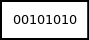
\includegraphics[scale=0.6]{img/chromosome.png}
\caption{Chromosome representation as a binary string}\label{fig:chromosome}
\end{figure}

\subsection{Fitness Function}


\newpage
\bibliographystyle{plain}
\bibliography{citations}
\end{document}
